\documentclass[]{elsarticle} %review=doublespace preprint=single 5p=2 column
%%% Begin My package additions %%%%%%%%%%%%%%%%%%%
\usepackage[hyphens]{url}

  \journal{Which journal? Journal of Service Research/Health Services Research/EJOR/IJF} % Sets Journal name


\usepackage{lineno} % add
\providecommand{\tightlist}{%
  \setlength{\itemsep}{0pt}\setlength{\parskip}{0pt}}

\usepackage{graphicx}
\usepackage{booktabs} % book-quality tables
%%%%%%%%%%%%%%%% end my additions to header

\usepackage[T1]{fontenc}
\usepackage{lmodern}
\usepackage{amssymb,amsmath}
\usepackage{ifxetex,ifluatex}
\usepackage{fixltx2e} % provides \textsubscript
% use upquote if available, for straight quotes in verbatim environments
\IfFileExists{upquote.sty}{\usepackage{upquote}}{}
\ifnum 0\ifxetex 1\fi\ifluatex 1\fi=0 % if pdftex
  \usepackage[utf8]{inputenc}
\else % if luatex or xelatex
  \usepackage{fontspec}
  \ifxetex
    \usepackage{xltxtra,xunicode}
  \fi
  \defaultfontfeatures{Mapping=tex-text,Scale=MatchLowercase}
  \newcommand{\euro}{€}
\fi
% use microtype if available
\IfFileExists{microtype.sty}{\usepackage{microtype}}{}
\usepackage[top=25mm, left=30mm, right=30mm, bottom=25mm,headsep=10mm, footskip=12mm]{geometry}
\usepackage{natbib}
\bibliographystyle{plainnat}
\usepackage{longtable}
\ifxetex
  \usepackage[setpagesize=false, % page size defined by xetex
              unicode=false, % unicode breaks when used with xetex
              xetex]{hyperref}
\else
  \usepackage[unicode=true]{hyperref}
\fi
\hypersetup{breaklinks=true,
            bookmarks=true,
            pdfauthor={},
            pdftitle={Short-term hourly forecasting for care services},
            colorlinks=false,
            urlcolor=blue,
            linkcolor=magenta,
            pdfborder={0 0 0}}
\urlstyle{same}  % don't use monospace font for urls

\setcounter{secnumdepth}{5}
% Pandoc toggle for numbering sections (defaults to be off)


% Pandoc header
\usepackage{adjustbox, float,lscape}



\begin{document}
\begin{frontmatter}

  \title{Short-term hourly forecasting for care services}
    \author[University1]{Author1\corref{1}}
   \ead{email1@example.com} 
    \author[University2]{Author2\corref{2}}
   \ead{email2@example.com} 
    \author[University3]{Author3\corref{2}}
   \ead{email3@example.com} 
      \address[University1]{Cardiff business school, 3 Colum Drive, CF10 3EU, Cardiff}
    \address[University2]{adress2}
    \address[University3]{adress3}
      \cortext[1]{Corresponding Author}
    \cortext[2]{Equal contribution}
  
  \begin{abstract}
  The Objective of this work would be to propose a new methodology to forecast short-term hourly forecasting for urgent and emergency care.
  \end{abstract}
  
 \end{frontmatter}

\hypertarget{introduction}{%
\section{Introduction}\label{introduction}}

why forecasting for urgent and emergency care is important?

Urgent and emergency healthcare is increasingly regarding patients as consumers of its service and aims to provide `consumer satisfaction'; particularly in the Accident and Emergency (A\&E) department and Ambulance services which have been viewed as the `shop window' of the hospital service. An accurate forecasting of the demand is essential in A\&E and Ambulance service trust to depict various courses of action that can result in massive savings in terms of patient lives.

Accurate forecasts contribute to better allocation of resources. Patient overcrowding in urgent and emergency care is a serious problem that causes challenging situations on patient flow . Also, it is related with increasing length of stay (LOS), low patient satisfaction about treatments on patients, number of patients left the ED without seen by medical staff , unexpected return visits to EDs , increasing health care costs and some other miscellaneous problems such as inaccuracy in electronic medical record-reported wait times to initial emergency physician evaluation and nursing staff requirement!

why hourly forecast is important?

12 hour forecasts are required to inform the Operations Department and in particular the Operational Delivery Unit (ODU) of future demand, particularly for the current and the next shift. The combination of forecast demand, incidents being attended, resource availability and delays at hospital provide information on the state of the unscheduled care system across Wales. Having this full picture enables the ODU to focus on the areas that require intervention to enable the most effective delivery of the service to the patients of Wales.

Forecasting hourly admissions is crucial for operational planning which involves the short-term decision making related to the execution of the delivery process for various health care services such as Ambulatory ,Emergency, Surgical, Inpatient, Home and Residential.

\begin{itemize}
\tightlist
\item
  Adjusting the Schedule during a day or a week because of unplanned events, such as emergency or walk-in patients, extended consultation times, and equipment
\item
  Dynamic patient (re)assignment
\item
  Staff rescheduling At the start of a shift, the staff sche- dule is reconsidered. Before and during the shift, the staff capacities may be adjusted to unpredicted demand fluctuations and staff absenteeism by using part-time, on- call nurses, staff overtime and voluntary absenteeism
\end{itemize}

what literature says about hourly forecasting in healthcare?

There exists a large literature on forecasting patient arrival, however the variation in arrivals remain unaccounted for. The forecasted hourly admissions at a typical A\&E or Ambulance service show a mean absolute percentage error (MAPE) of 50\%. Hourly forecasts are challenging because the noise caused by random variation may overshadow any pattern in the data. In this respect, forecasts of daily or monthly arrivals are likely easier but target decisions about staff allocation and the like, not the ongoing scheduling and rescheduling of how the available resources are divided among the patients in need of emergency services

limitations in current literature?

how we add to the literature?

Our contributions are as following:

\begin{enumerate}
\def\labelenumi{\arabic{enumi}.}
\tightlist
\item
  We develope a novel methodology to forecast hourly time series for healthcare services combining a distributio fit to each hour of day seperately and then adjust it using variables accounting for i) trend, ii) autocorrelation iii) temporal factors such as day of week, \ldots{} iv) special events such as public holidays, festive days and rugby and v) weather data.
\item
  We provide prbabilistic forecasts \ldots{}
\item
  We benchmark the forecasting performance of the proposed methodology against regression, prophet and TBATS using \ldots{}.
\end{enumerate}

The rest of the paper is organised as following: section \ref{lit} provides a brief overview of the use of temporal aggregation in time series forecasting. Section \ref{model} starts with \ldots{}

\hypertarget{lit}{%
\section{Research background: Hourly forecasting in care services}\label{lit}}

\begin{table}[h]
\caption{Summary of studies in hourly emergency care forecasting}
\centering 
\begin{adjustbox}{width=1\textwidth}
\small

\begin{tabular}{clllll} 
\hline
Authors & What to forecast & Method & Forecast evaluation & Limitations  \\ 
\hline 

\citet{hertzum2017forecasting} & Hourly ED patient arrivals and ED occupancy forecasting using calendar variables  1-3 & Regression, ARIMA, naive & MAPE & blabla\\ 
\citet{mccarthy2008challenge} & To develop methodology for predicting demand for ED services by characterizing ED arrivals  1-3 & Poisson regression & RMSE & blabla\\ 
\citet{morzuch2006forecasting} & hourly ED arrivals for 24 hours & Holt-Winters & MAPE & blabla\\ 
\citet{chase2012predicting} & ED volume & Logistic regression & RMSE & blabla\\ 
\citet{jones2009multivariate} & Demands for key resources in the ED and the inpatient hospital  & S, ARIMA & RMSE & blabla\\ 


\hline
\end{tabular}
\end{adjustbox}
\label{tab:lit-summary}
\end{table}

Table \ref{tab:lit-summary} summarise studies in hourly forecasting in emergency and urgent care.

Linear regression, ARIMA, and naive models were used by \citet{hertzum2017forecasting} to investigate whether accurate hourly accident and emergency department patient arrivals and occupancy forecasts can be generated using calendar variables. Naive model was there for the purpose of comparison. \citet{hertzum2017forecasting} study shows that patient arrivals variation is larger across the hours of the day than across the days of the week and the months of the year. In term of hour of the day, patient arrivals peaked around noon. For days of the week, Monday is the busiest day while weekends are the quietest days. July-August are the month with the highest number of patient arrivals and January and February are the months with the lowest number of arrivals. The regression and ARIMA models perform similarly for all forecast interval in modeling patient arrivals. In modeling accident and emergency department occupancy, ARIMA outperform regression models. However, after all, the models of occupancy were less accurate than those arrivals. \citet{hertzum2017forecasting} mentioned that ARIMA models are among the most accurate models for accident and emergency department visits forecasting. Another interesting point is that the accuracy of accident and emergency department forecasting models decrease with the increasing forecast interval. Lastly, the accuracy of the forecasting model may possibly be increased with additional information added to the model.

Predicting the arrivals of accident and emergency department future patients is studied by \citet{choudhury2020forecasting} ARIMA, Holt-Winters, TBATS, and neutral network methods were implemented to forecast hourly accident and emergency department arrivals. ARIMA model was selected as the best fit model and it has provided high and acceptable hourly accident and emergency department forecasting accuracy. \citet{hertzum2017forecasting} work was mentioned in this paper. It is said that residual normality, stationarity, and autocorrelation have not been tested in \citet{hertzum2017forecasting} paper and this might be the cause of accuracy problems. However, residual normality, stationarity, and autocorrelation are tested and compared with Holt-Winters, TBATS, and neutral network methods in \citet{choudhury2020forecasting}
According to the studies mentioned earlier, it can be said that the existing studies have shown complications in forecasting hourly patient accident and emergency department visits and the application of forecasting hourly patients visits is not well established. Some of the studies said that the accuracy of hourly accident and emergency department forecasting model is low compared to other longer forecasting intervals like daily forecast \citep{boyle2012predicting, hertzum2017forecasting}. However, some studies mentioned that the accuracy of accident and emergency department hourly forecast is at the acceptable level \citep{choudhury2020forecasting, mccarthy2008challenge, schweigler2009forecasting}.

The literature review reveals some limitations in forecasting for urgent and emergency care which will be summarised as follows:

\begin{itemize}
\tightlist
\item
  first,
\item
  second,
\item
  third,
\end{itemize}

\hypertarget{model}{%
\section{Proposed model}\label{model}}

\hypertarget{design}{%
\section{Experimental design}\label{design}}

\hypertarget{data}{%
\subsection{data}\label{data}}

Figure \ref{fig:hourly-plot}

Figure \ref{fig:24hour}

\begin{figure}[H]

{\centering 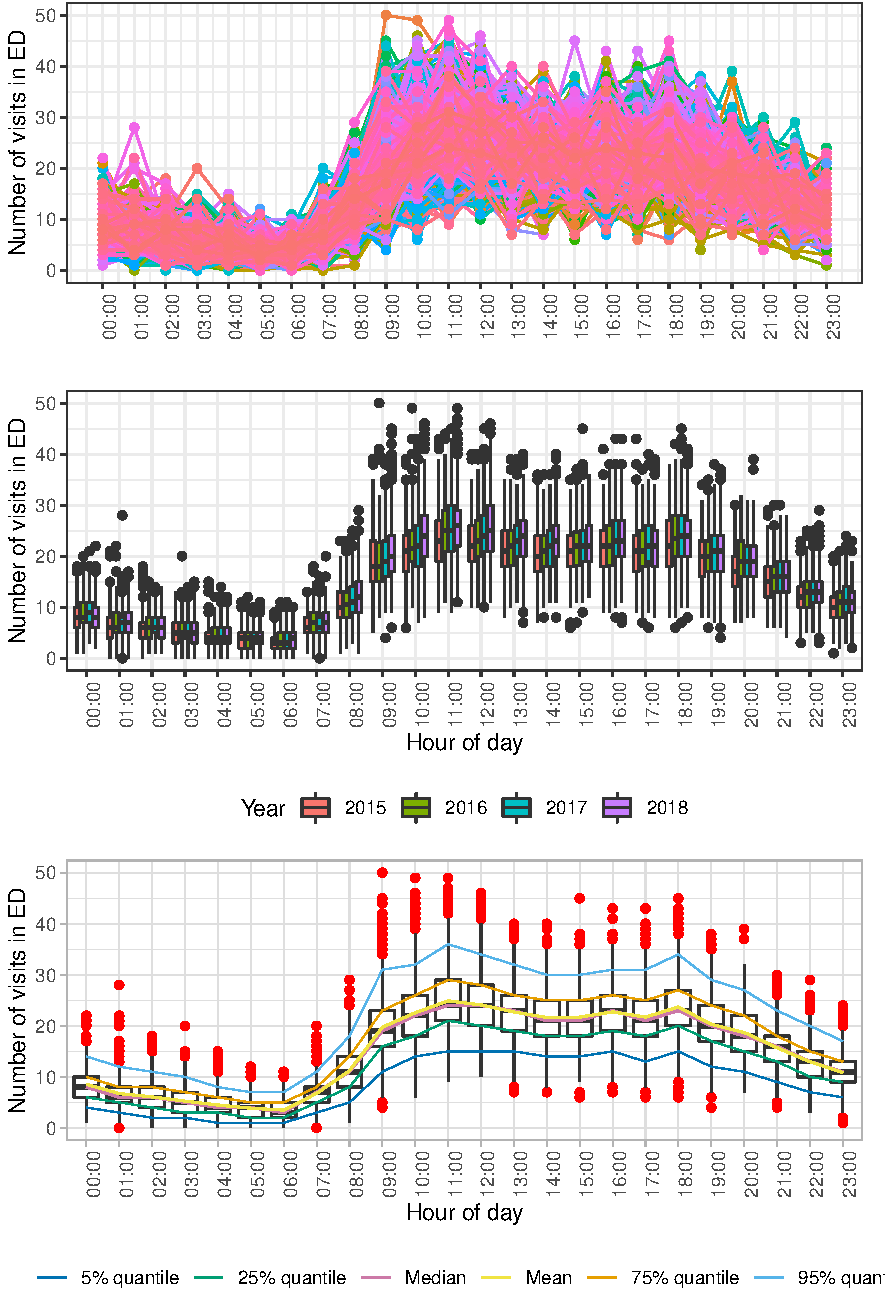
\includegraphics{paper_files/figure-latex/hourly-plot-1} 

}

\caption{Seasonal plot of ED attendance}\label{fig:hourly-plot}
\end{figure}

\begin{figure}[H]

{\centering 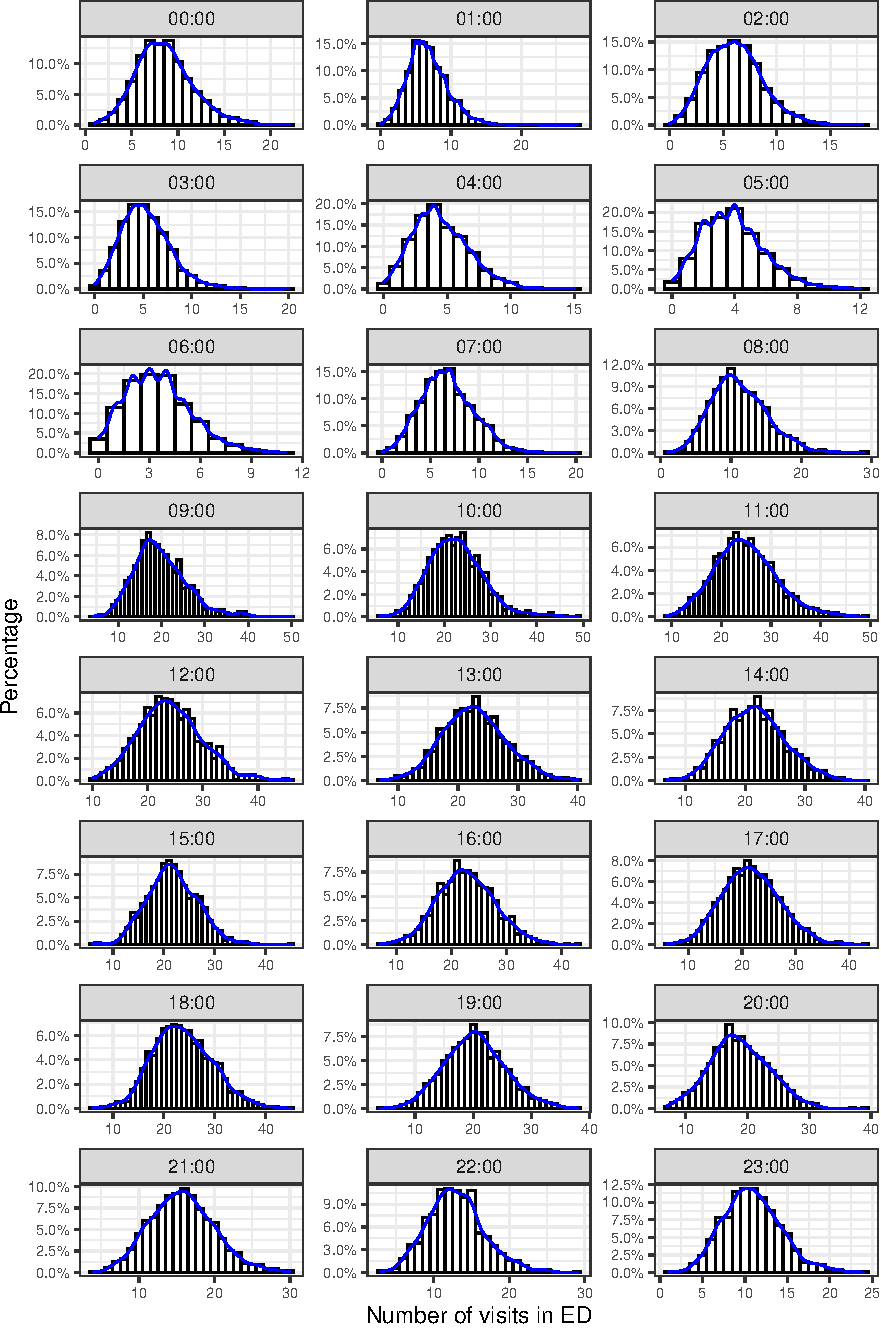
\includegraphics{paper_files/figure-latex/24hour-1} 

}

\caption{Distrubution of ED attendance for each hour of day}\label{fig:24hour}
\end{figure}

\hypertarget{benchmarks}{%
\subsection{benchmarks}\label{benchmarks}}

\begin{equation}
\bar{X} = \frac{\sum_{i=1}^n X_i}{n} \label{eq:mean}
\end{equation}

Also see Equation \eqref{eq:mean}

\hypertarget{accuracy}{%
\subsection{forecast performance evaluation}\label{accuracy}}

\hypertarget{result}{%
\section{Result and discussion}\label{result}}

\hypertarget{conclusion}{%
\section{Conclusion}\label{conclusion}}

\renewcommand\refname{References}
\bibliography{mybibfile.bib}


\end{document}


